\chapter{Architecture Description}
\index{Architecture Description}
\label{chap:ad}
This chapter provides a summary of the research done for this thesis as an resulting artefact. This artefact takes the form of an architecture description in accordance to ISO42010 and is expressed in terms of the 4+1 view model.

\section{The 4+1 View of our Architecture}


\subsection{Scenario View (Use Case View)}

\begin{table}[h]
\centering
\begin{tabularx}{\textwidth}{lXl}
\cline{1-2}
\multicolumn{2}{|c|}{\cellcolor[HTML]{EFEFEF}Scenario View} &  \\ \cline{1-2}
\multicolumn{1}{|l|}{Figure \ref{fig:coreusecase}} & \multicolumn{1}{X|}{Figure \ref{fig:coreusecase} is used to illustrate the basic functional requirements of the system as a use case. It shows the interaction between the three main actors in our system.} &  \\ \cline{1-2}
\multicolumn{1}{|l|}{Figure \ref{fig:tenantusecase}} & \multicolumn{1}{X|}{In addition to the core "marketplace" related use cases for our system, an additional high level use case for provisioning new tenants is outlined by figure \ref{fig:tenantusecase}.} & \\
\cline{1-2}
\end{tabularx}
\caption{Scenario View}
\label{my-label}
\end{table}




\begin{figure}
\centering
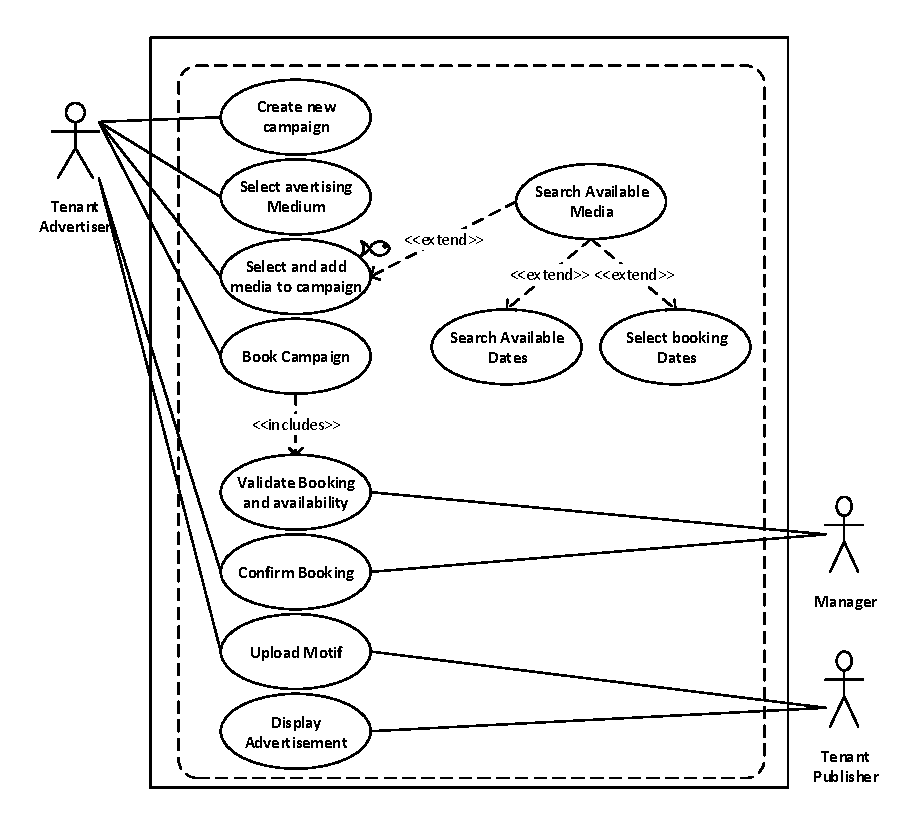
\includegraphics[width=\textwidth]{CoreUseCase}
\caption{Functional Use Case}
\label{fig:coreusecase}
\end{figure}


\begin{figure}
\centering
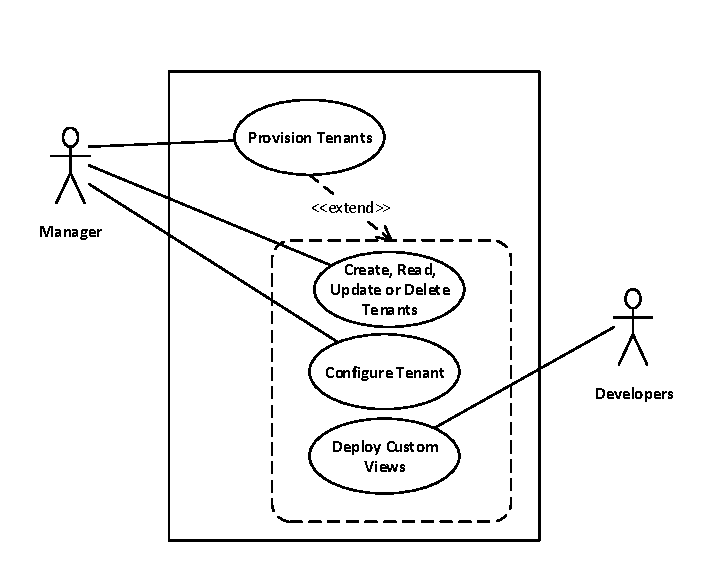
\includegraphics[width=\textwidth]{TenantUseCase}
\caption{Tenant Provisioning Use Case}
\label{fig:tenantusecase}
\end{figure}

\section{Logical View (Object View)}

\begin{table}[h]
\centering
\begin{tabularx}{\textwidth}{lXl}
\cline{1-2}
\multicolumn{2}{|c|}{\cellcolor[HTML]{EFEFEF}{\color[HTML]{000000} Logical View}} &  \\ \cline{1-2}
\multicolumn{1}{|l|}{Figure \ref{fig:marketclass}} & \multicolumn{1}{X|}{Figure \ref{fig:marketclass} shows the class diagram for our marketplace context. It shows the different classes that can be used in order to satisfy our functional requirements. It also shows the relationship between these classes. It is important to articulate the inclusion of two abstract classes nl. \textit{AzureSearchResource} and \textit{AzureDocumentResource}. These two classes are provided by the AzureDocumentDB and AzureSearch components and are required by all objects that need to be persisted by either technology.} &  \\ \cline{1-2}
\multicolumn{1}{|l|}{Figure \ref{fig:infraclass}} & \multicolumn{1}{X|}{Figure \ref{fig:infraclass} has been created in order to provide implementation level details of the patterns suggested. This class diagram can be combined with the component and package diagrams in the AD to provide enough information to implement the basics of each pattern.} &  \\ \cline{1-2}
\cline{1-2}
\end{tabularx}
\caption{My caption}
\label{my-label}
\end{table}

%%%%%%%%%%% CLASS DIAGRAMS%%%%%%%%%%%%%%%%

\begin{figure}
\centering
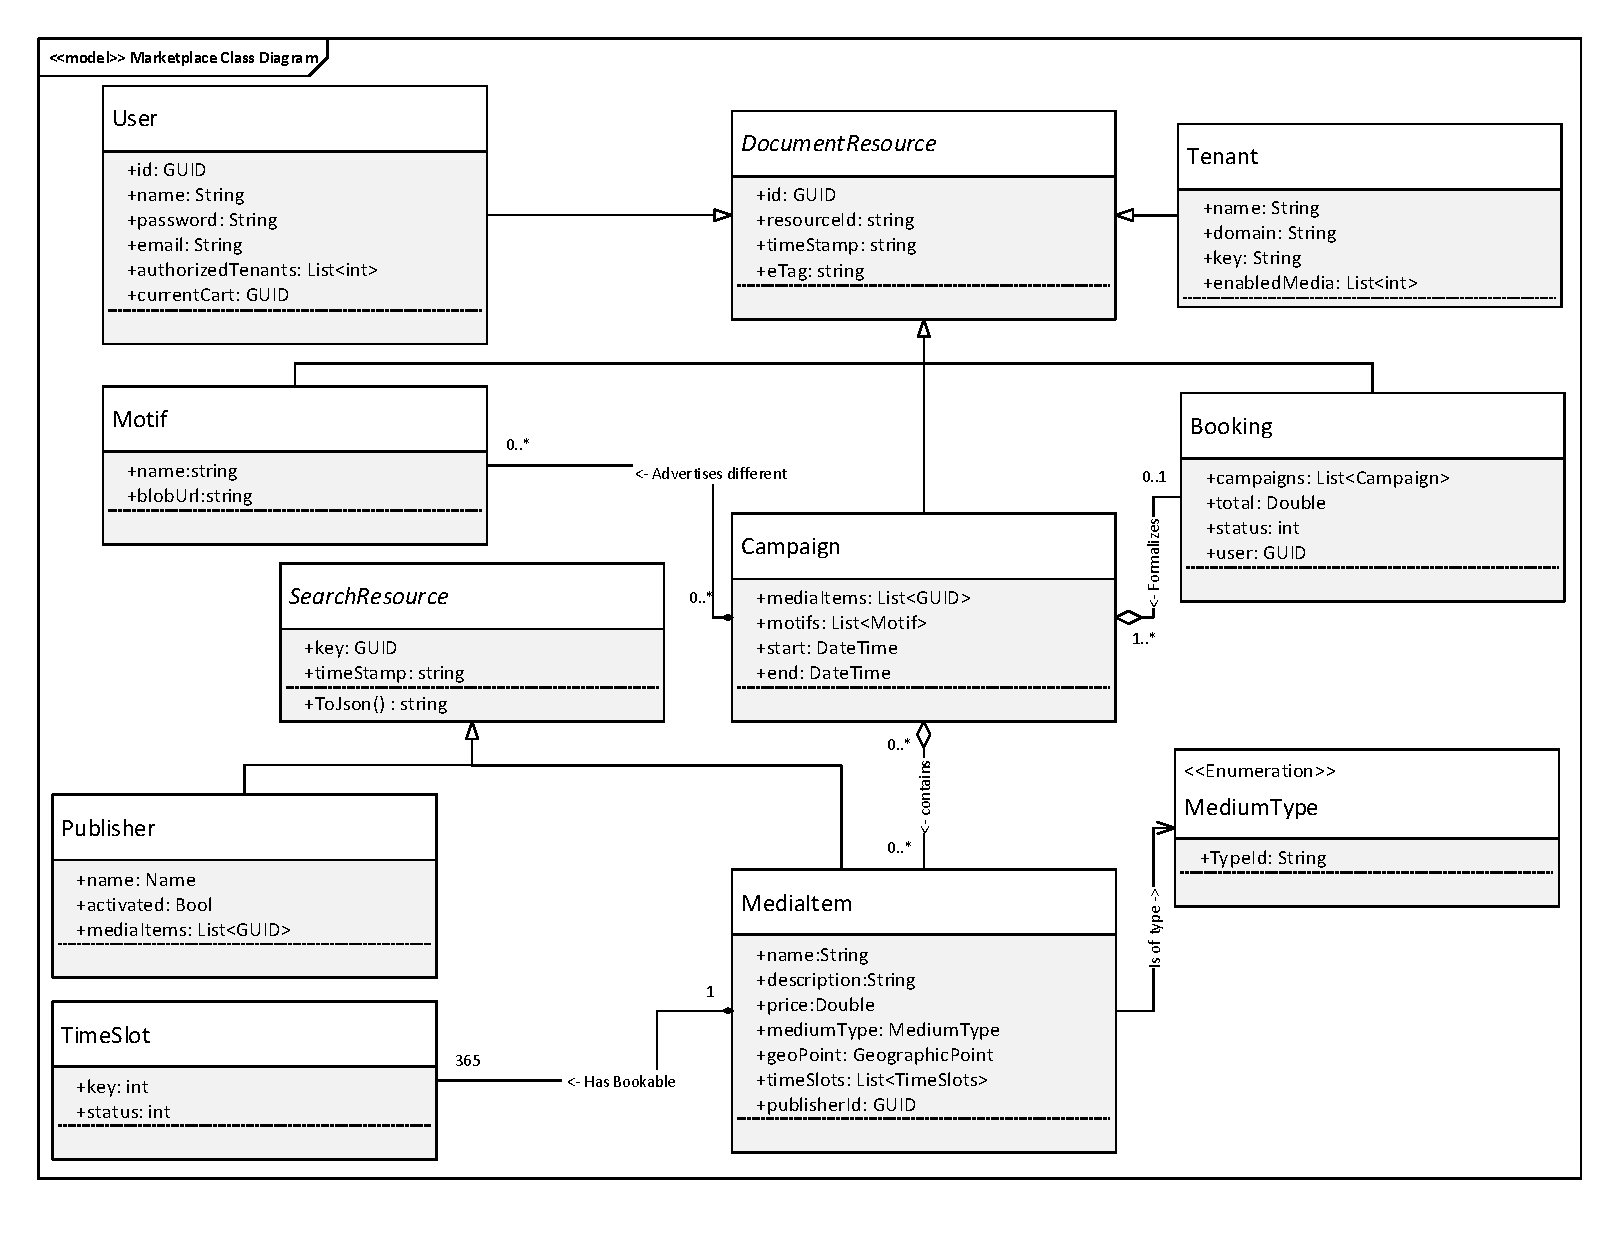
\includegraphics[width=\textwidth]{MarketplaceClassDiagram}
\caption{Marketplace Class Diagram}
\label{fig:marketclass}
\end{figure}


\begin{figure}
\centering
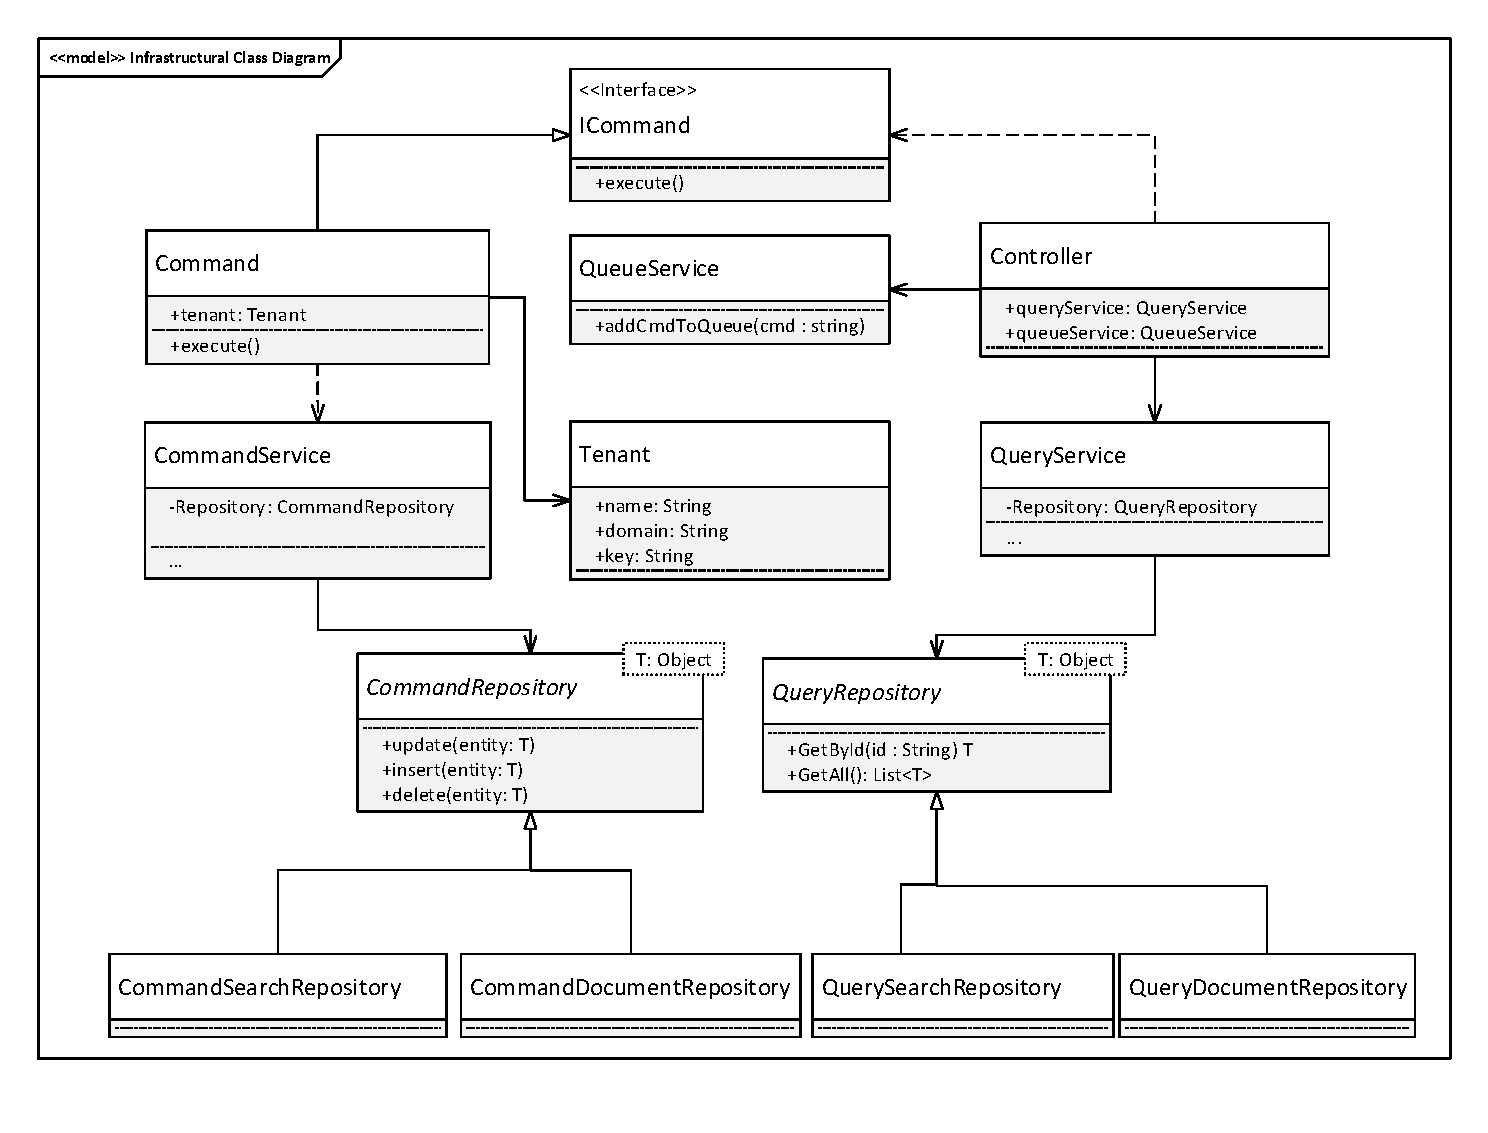
\includegraphics[width=\textwidth]{InfrastructuralClassDiagram}
\caption{Infrastructural Class Diagram}
\label{fig:infraclass}
\end{figure}


\section{Process View}

\begin{table}[h]
\centering
\begin{tabularx}{\textwidth}{lXl}
\cline{1-2}
\multicolumn{2}{|c|}{\cellcolor[HTML]{EFEFEF}Process View} &  \\ \cline{1-2}
\multicolumn{1}{|X|}{\begin{tabular}[c]{@{}l@{}}Figure\ref{fig:commandissuesequencediagram}, \\ Figure \ref{fig:commandhandlesequencediagram}\end{tabular}} & \multicolumn{1}{l|}{The following diagram (\ref{fig:commandissuesequencediagram} \& \ref{fig:commandhandlesequencediagram}) outlines the activity flows for commands. This flow would be followed by any request that requires the modification of database data. It is important to note how this applies the command and QCW \index{Queue Centric Workflow} patterns and completely separates the front end from the queue handler.} &  \\ \cline{1-2}
\multicolumn{1}{|l|}{Figure \ref{fig:activitydiagram}} & \multicolumn{1}{l|}{The activity diagram in figure \ref{fig:activitydiagram} outlines the entire workflow of activities in our marketplace. It highlights the different functional requirements in terms of activities as well as decision points along the flow.} &  \\ \cline{1-2}
\multicolumn{1}{|l|}{Figure \ref{fig:activitytenantisolation}} & \multicolumn{1}{l|}{The Dual Input/Tenant Validation pattern has been suggested for addressing tenant data isolation. The flow for implementing this pattern is shown in figure \ref{fig:activitytenantisolation}.} &  \\ \cline{1-2}
 &  &  \\ \cline{1-2}
\cline{1-2}
\end{tabularx}
\caption{My caption}
\label{my-label}
\end{table}

%%%%%%%% SEQUENCE DIAGRAMS%%%%%%%%%%%%%%%%

\begin{figure}
\centering
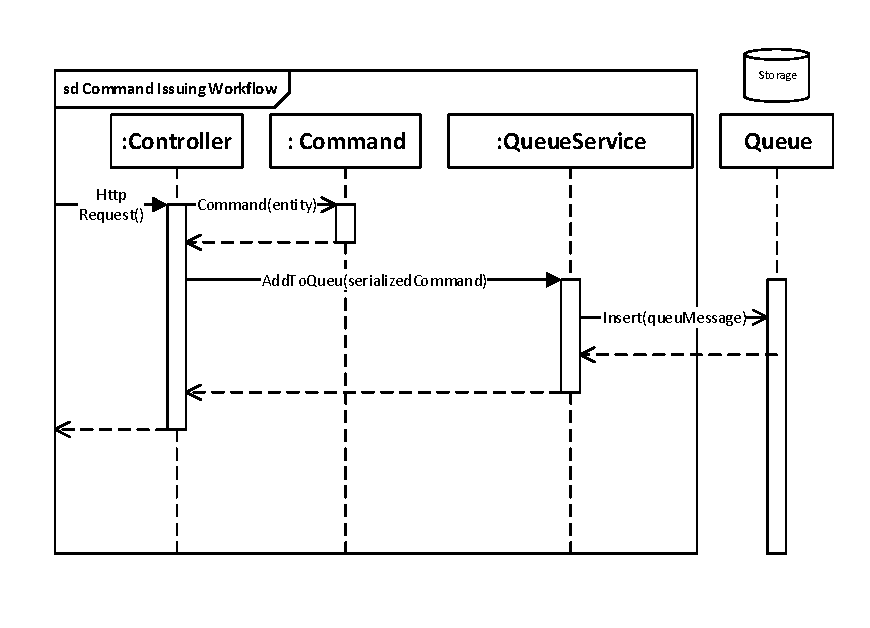
\includegraphics[width=\textwidth]{CommandIssueSequenceDiagram}
\caption{Command Issue Sequence Diagram}
\label{fig:commandissuesequencediagram}
\end{figure}

\begin{figure}
\centering
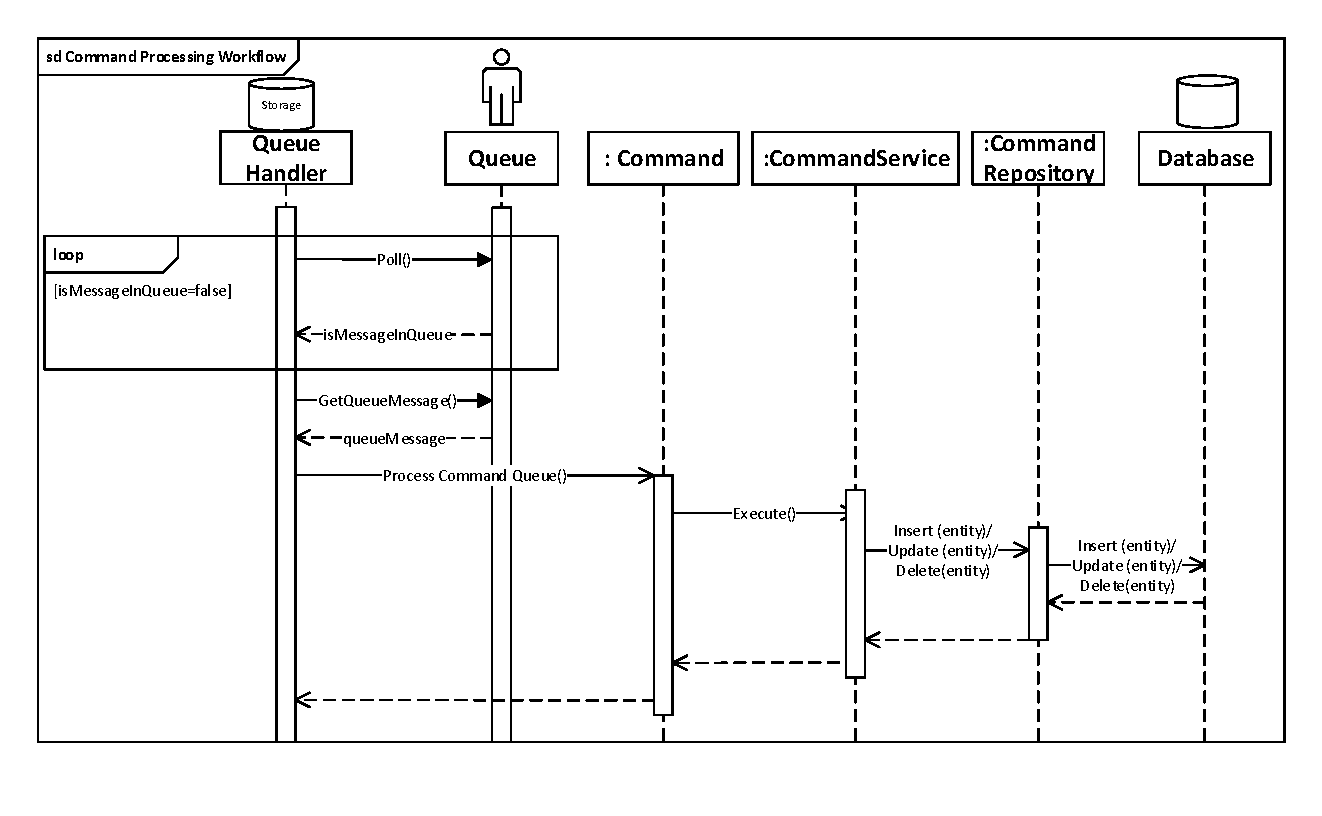
\includegraphics[width=\textwidth]{CommandOnlySequenceDiagram}
\caption{Command Handling Sequence Diagram}
\label{fig:commandhandlesequencediagram}
\end{figure}


%%%%%%%% ACTIVITY DIAGRAMS %%%%%%%%%%%%%%%
\subsection{Marketplace Activity Flow}

\begin{figure}
\centering
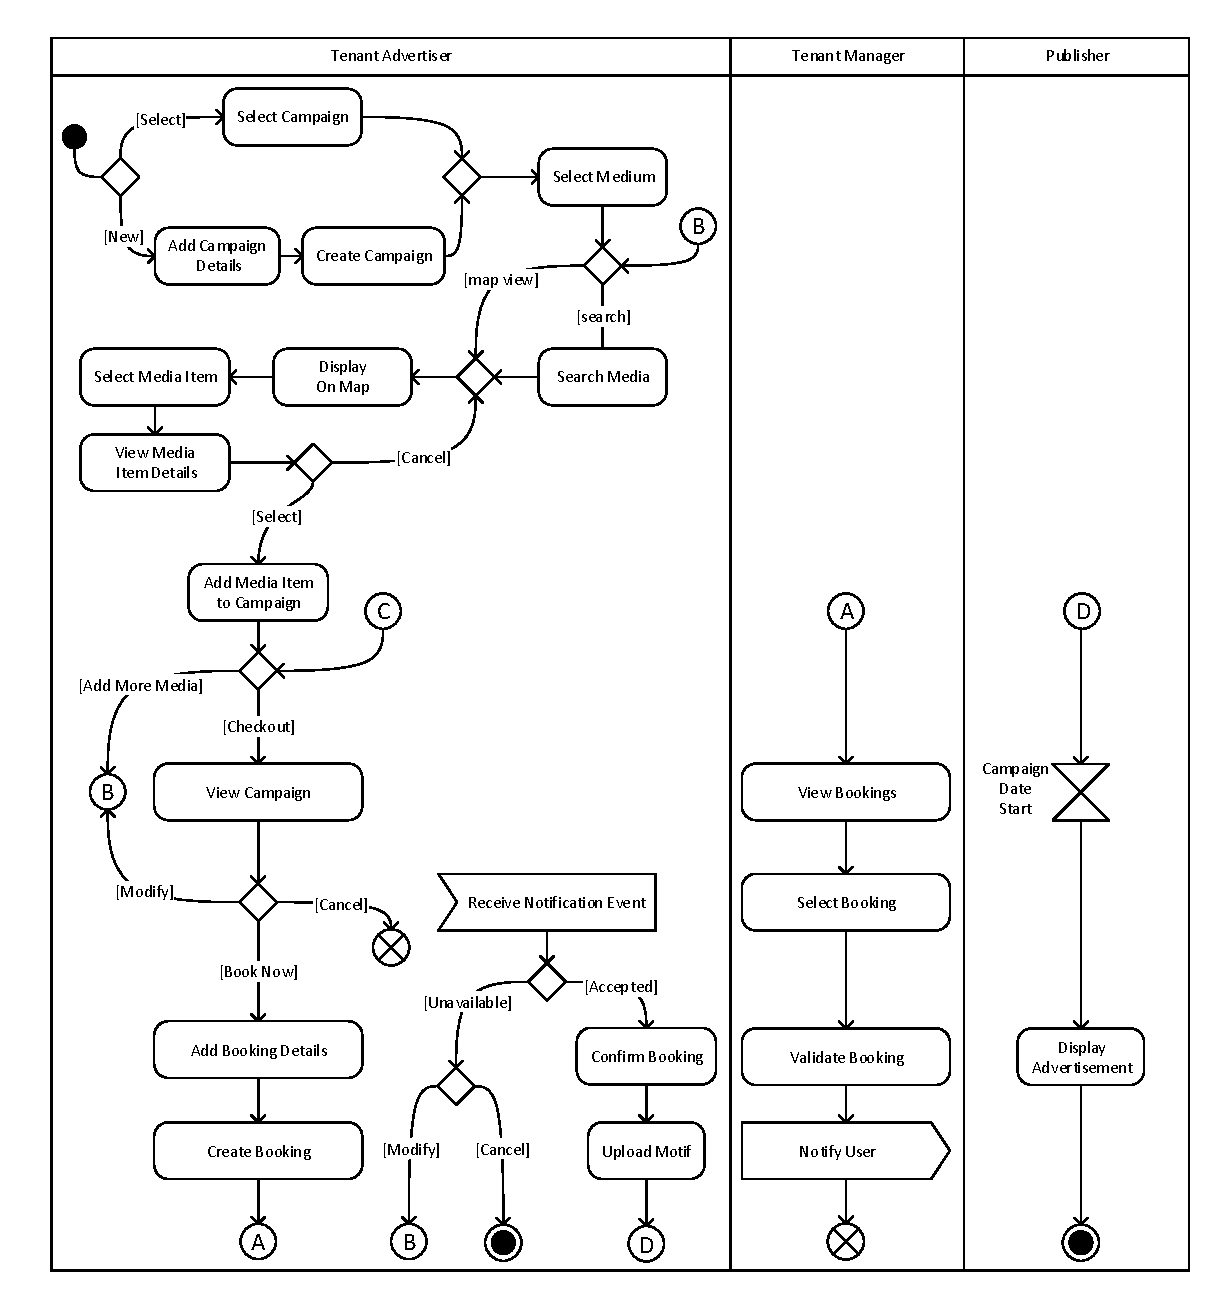
\includegraphics[width=\textwidth]{ActivityDiagram}
\caption{Marketplace Activity Diagram}
\label{fig:activitydiagram}
\end{figure}

\begin{figure}
\centering
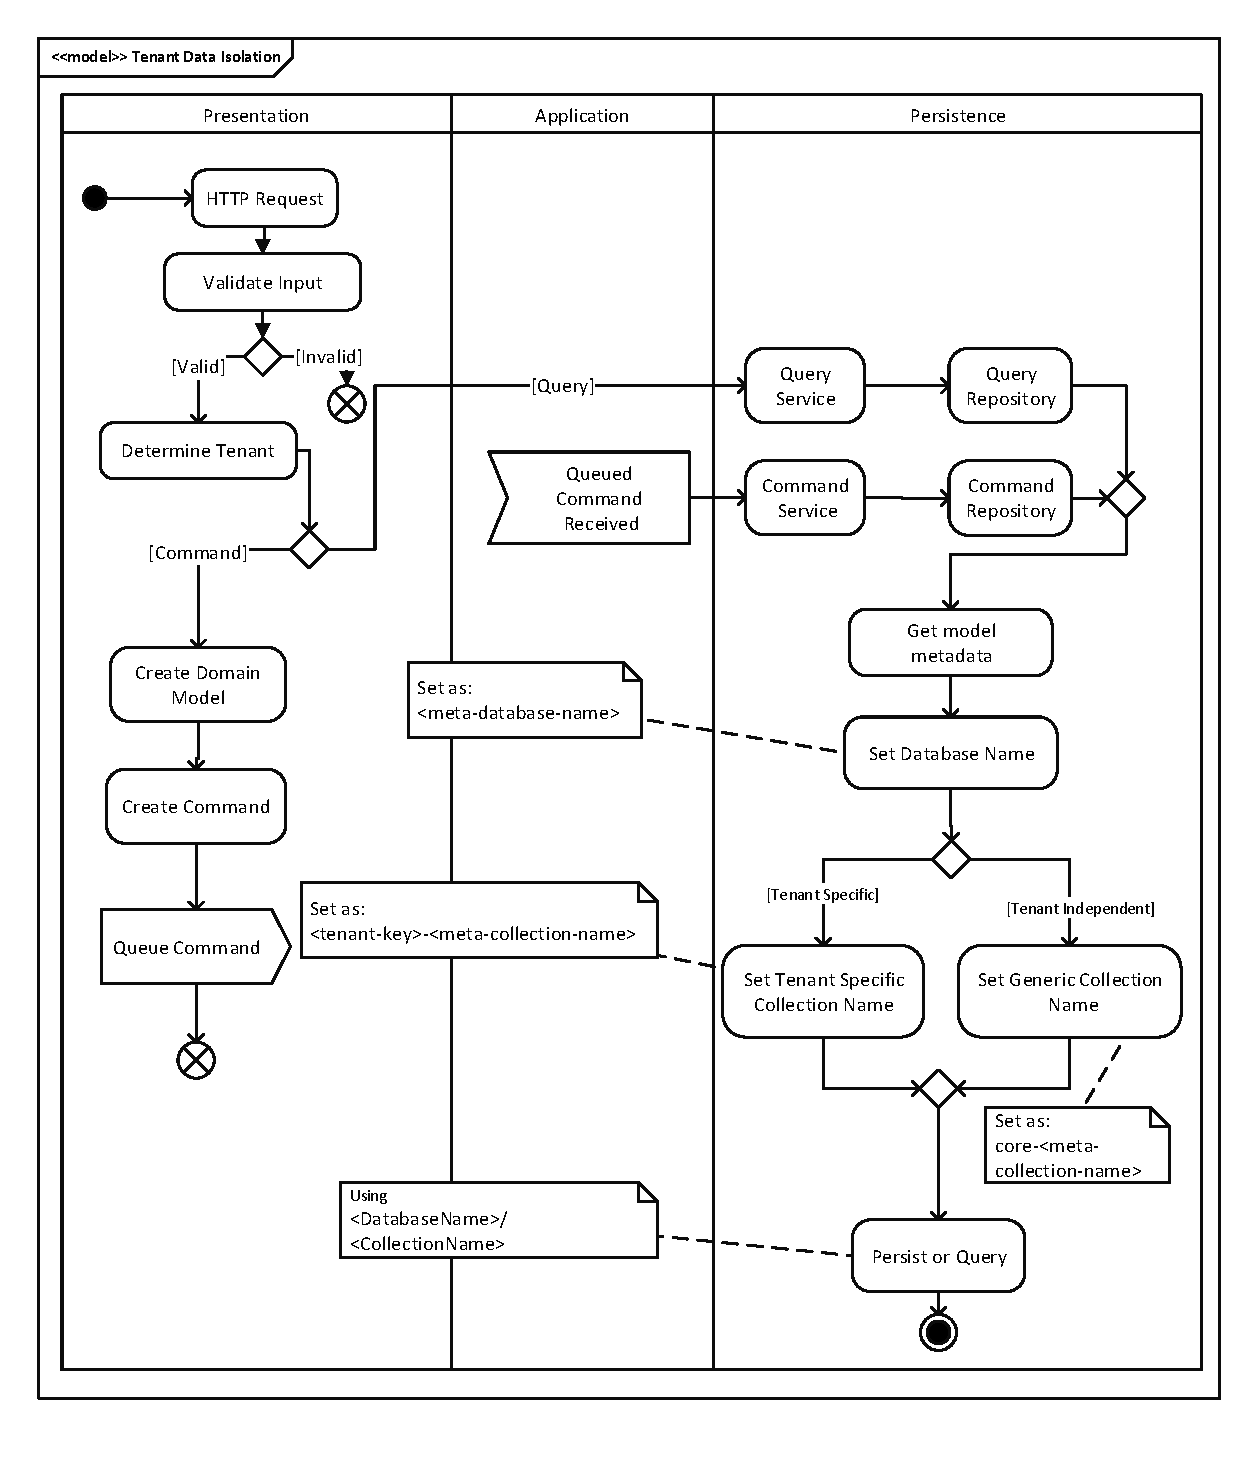
\includegraphics[width=\textwidth]{ActivityDiagramStorage}
\caption{Tenant Data Isolation Activity Diagram}
\label{fig:activitytenantisolation}
\end{figure}



\section {Development View (Implementation View)}

\begin{table}[h]
\centering
\begin{tabularx}{\textwidth}{lXl}
\cline{1-2}
\multicolumn{2}{|c|}{\cellcolor[HTML]{EFEFEF}Development View} &  \\ \cline{1-2}
\multicolumn{1}{|X|}{Figure \ref{fig:componentdiagram}} & \multicolumn{1}{l|}{In order to exemplify the different exchangeable components of our system a component diagram has been created. The model shown in figure \ref{fig:componentdiagram} indicates a high level overview of the encapsulated classes and the interfaces used for connecting these components. This diagram provides a broad overview of the system used for implementation.} &  \\ \cline{1-2}
\multicolumn{1}{|l|}{Figure \ref{fig:packagediagram}} & \multicolumn{1}{l|}{The package diagram shown in figure \ref{fig:packagediagram} emphasises the high level separation of different elements shown in figure \ref{fig:elements} as they divided into different packages.} &  \\ \cline{1-2}
 &  &  \\ \cline{1-2}
\cline{1-2}
\end{tabularx}
\caption{My caption}
\label{my-label}
\end{table}

%%%%%%%% COMPONENT DIAGRAMS %%%%%%%%%%%%%%

\begin{figure}
\centering
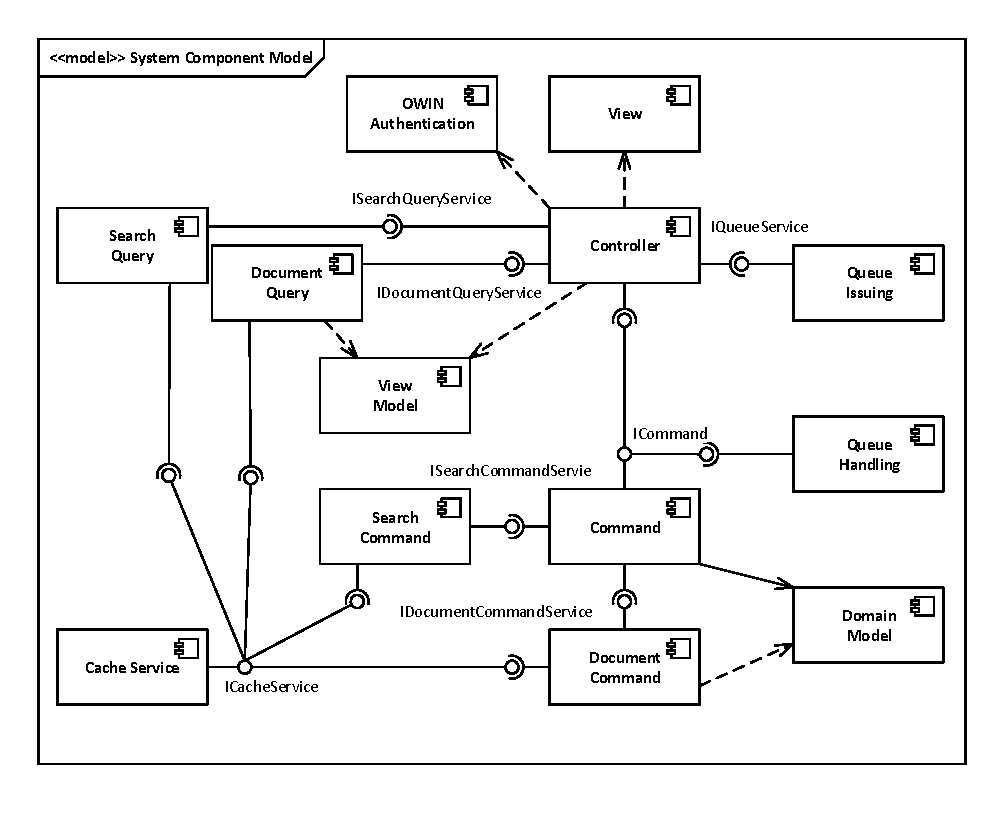
\includegraphics[width=\textwidth]{ComponentDiagram}
\caption{System Component Diagram}
\label{fig:componentdiagram}
\end{figure}

%%%%%%%% PACKAGE DIAGRAMS %%%%%%%%%%%%%%%%

\begin{figure}
\centering
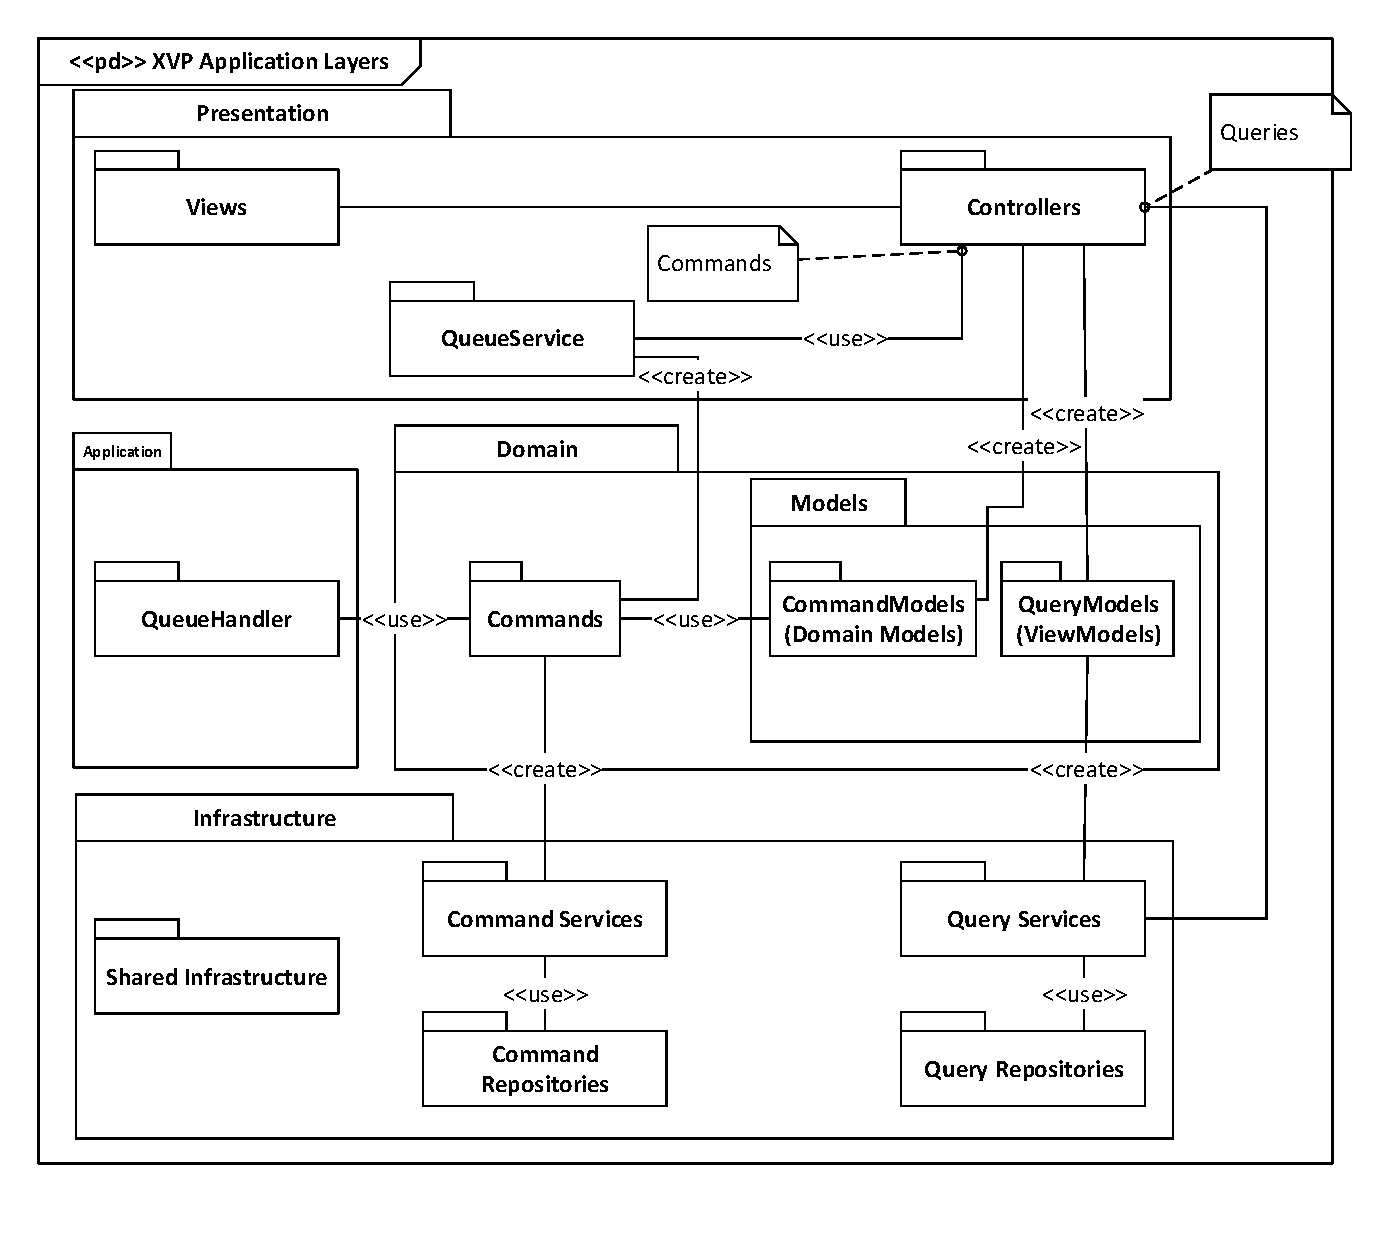
\includegraphics[width=\textwidth]{PackageDiagram}
\caption{Application Layering Package Diagram}
\label{fig:packagediagram}
\end{figure}


\section{Physical View (Deployment View)}

\begin{table}[h]
\centering
\begin{tabularx}{\textwidth}{lXl}
\cline{1-2}
\multicolumn{2}{|c|}{\cellcolor[HTML]{EFEFEF}Physical View} &  \\ \cline{1-2}
\multicolumn{1}{|X|}{Figure \ref{fig:deploymentdiagram}} & \multicolumn{1}{l|}{The deployment diagram depicted in figure \ref{fig:deploymentdiagram} gives the physical deployment of nodes within our multi-tenant system. It indicates the technologies, configurations and approaches chosen as a result of multi-tenancy for implementing our system. It is important to note that all network protocols have been omitted for simplicity.} &  \\ \cline{1-2}
\cline{1-2}
\end{tabularx}
\caption{My caption}
\label{my-label}
\end{table}

%%%%%%%% DEPLOYMENT DIAGRAMS %%%%%%%%%%%%%

\begin{figure}
\centering
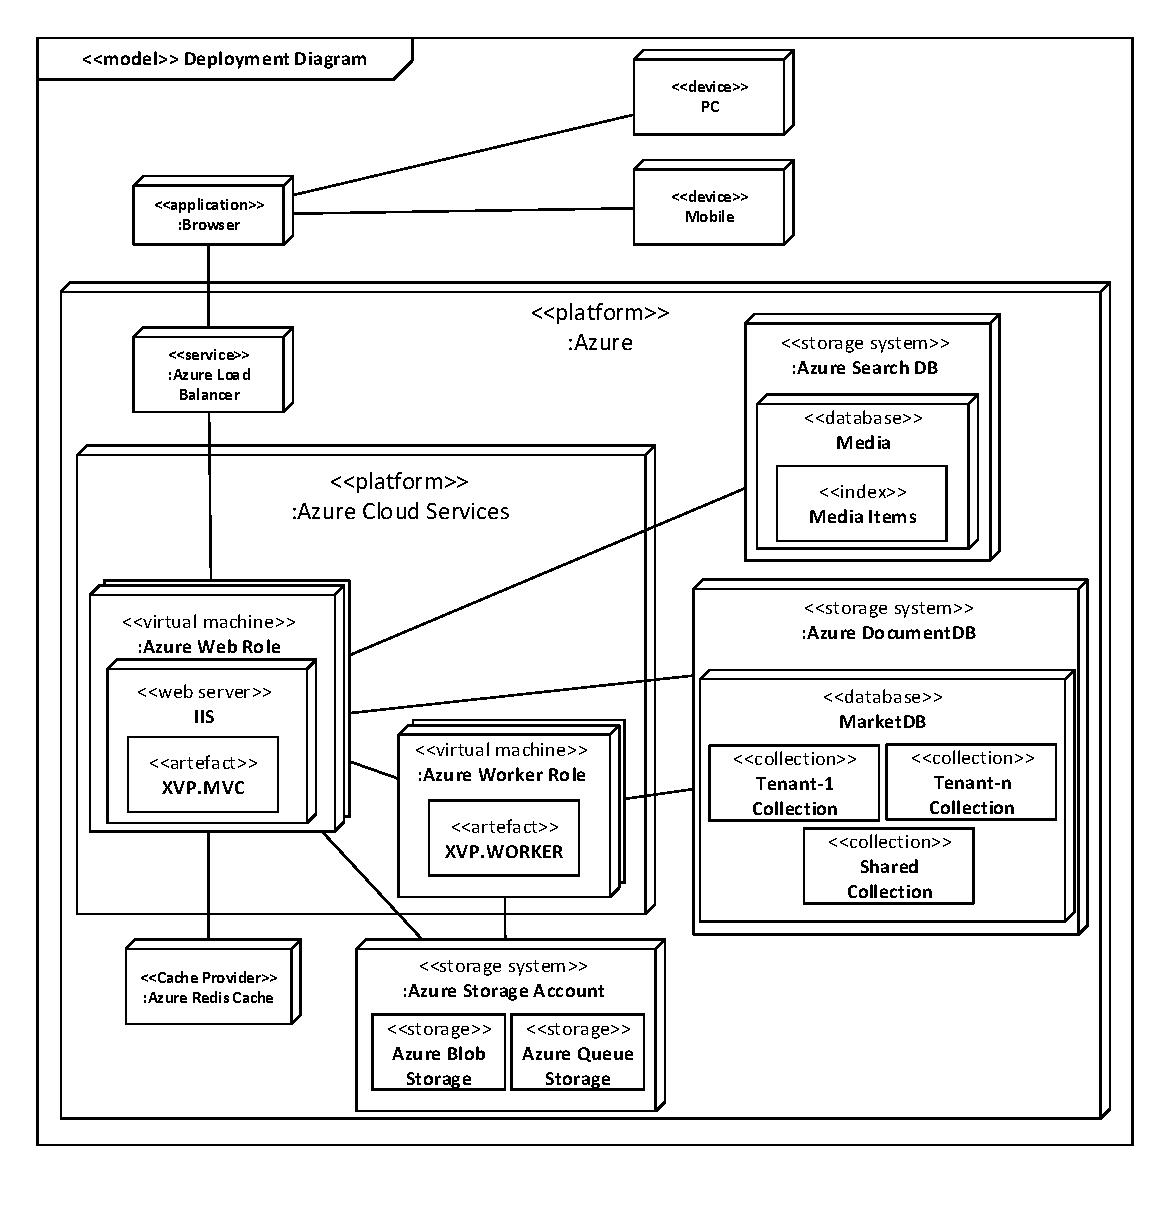
\includegraphics[width=\textwidth]{DeploymentDiagram}
\caption{Application Deployment Diagram}
\label{fig:deploymentdiagram}
\end{figure}
